\section{Aim}
 To study some basic SQL queries like, SELECT, INSERT, UPDATE, DELETE, and the WHERE clause.

\section{{Theory}}

\begin{itemize}
\item SELECT: Used to display the rows of a table. 
\item INSERT: Used to insert values into the table.
\item UPDATE: Used to update the values already inserted into the table based on the WHERE clause.
\item DELETE: Used to delete entries already inserted into the table based on the WHERE clause.
\item WHERE clause: Used to check for the presence or absence of a condition. 
\end{itemize}

\section{{Code and Output}}

\begin{enumerate}
\item Display the details of all the employees.\newline
\begin{minted}{sql}

SELECT * FROM employee

\end{minted}
\newline
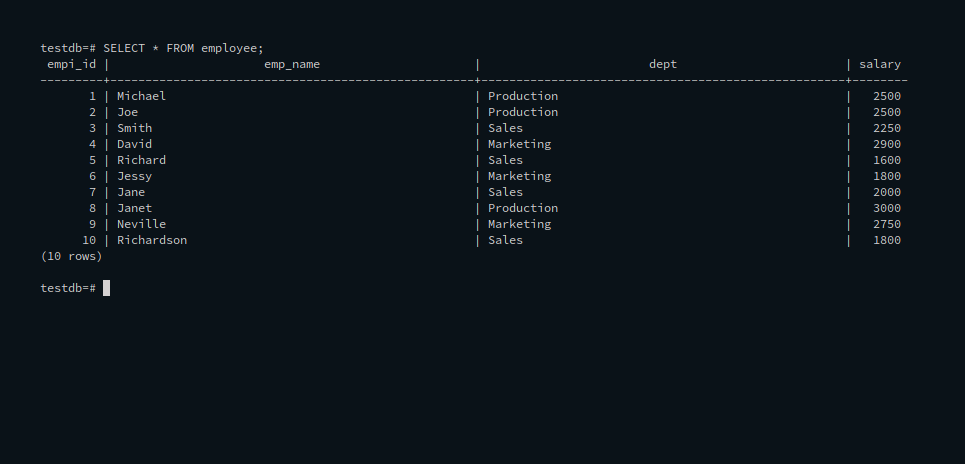
\includegraphics[width=\linewidth]{../Images/Basics/1.png}\newline
\item Display the names and id’s of all employees.\newline
\begin{minted}{sql}

SELECT emp_id, emp_name FROM employee;

\end{minted}
\newline
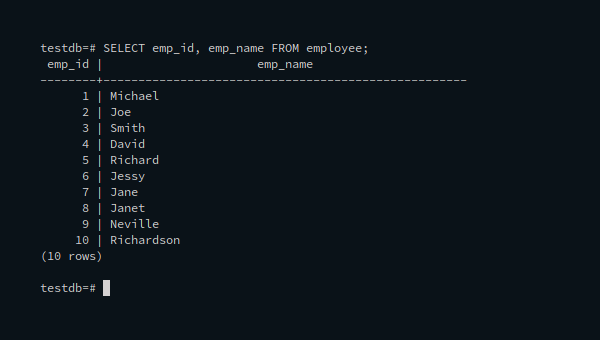
\includegraphics[width=\linewidth]{../Images/Basics/2.png}\newline
\item Delete the entry corresponding to employee id:10.\newline
\begin{minted}{sql}

DELETE FROM employee WHERE emp_id=10;

\end{minted}
\newline
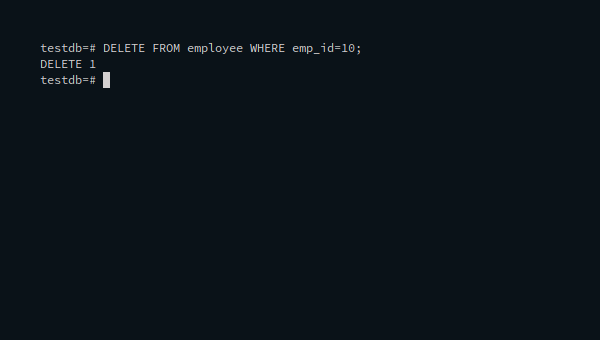
\includegraphics[width=\linewidth]{../Images/Basics/3.png}\newline
\item Insert a new tuple to the table. The salary field of the new employee should be kept NULL.\newline
\begin{minted}{sql}

INSERT INTO employee (emp_id, emp_name, dept) 
	VALUES (11, 'John', 'Sales');

\end{minted}
\newline
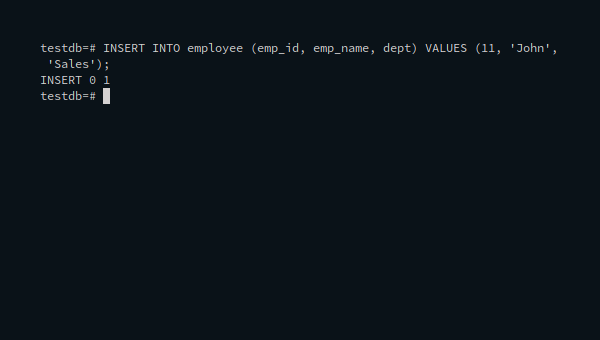
\includegraphics[width=\linewidth]{../Images/Basics/4.png}\newline
\item Find the details of all employees working in the marketing department.\newline
\begin{minted}{sql}

SELECT * FROM employee WHERE dept='Marketing';

\end{minted}
\newline
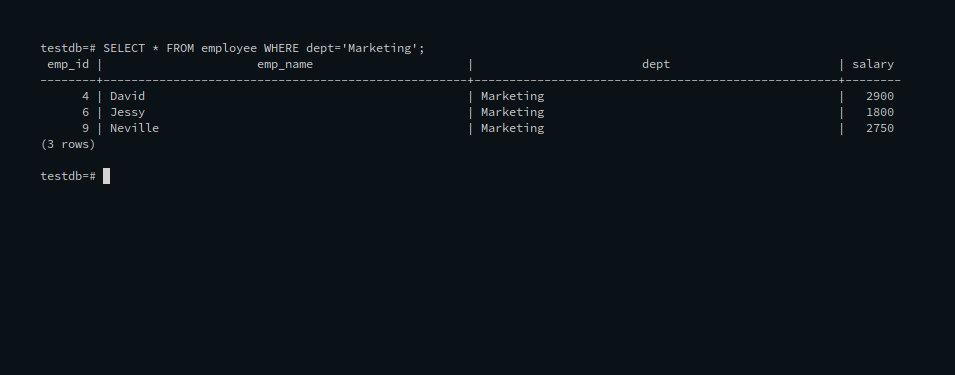
\includegraphics[width=\linewidth]{../Images/Basics/5.png}\newline
\item Add the salary details of the newly added employee.\newline
\begin{minted}{sql}

UPDATE employee SET salary = 1900 WHERE emp_id=10;

\end{minted}
\newline
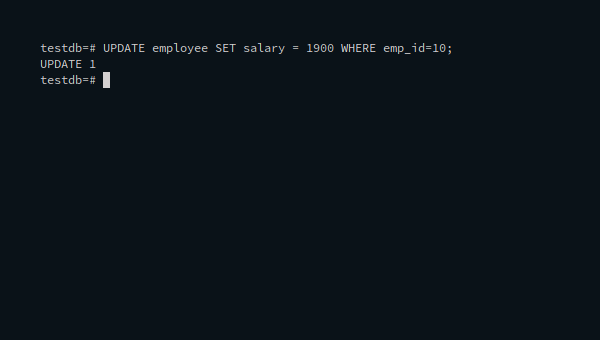
\includegraphics[width=\linewidth]{../Images/Basics/6.png}\newline
\item Update the salary of Richard to 1900\$.\newline
\begin{minted}{sql}

UPDATE employee SET salary = 1900 
	WHERE emp_name='Richard';

\end{minted}
\newline
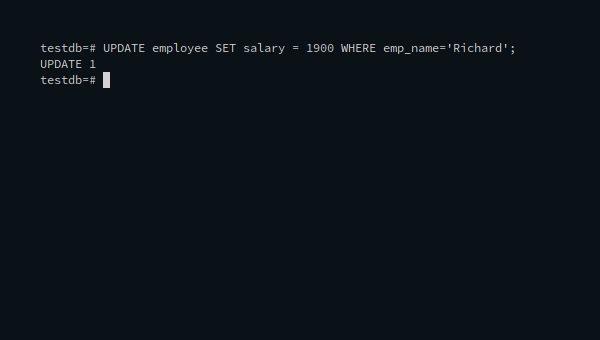
\includegraphics[width=\linewidth]{../Images/Basics/7.png}\newline
\item Find the details of all employees who are working for marketing and has a salary greater than	2000\$.\newline
\begin{minted}{sql}

SELECT * FROM employee 
	WHERE dept='Marketing' AND salary > 2000;

\end{minted}
\newline
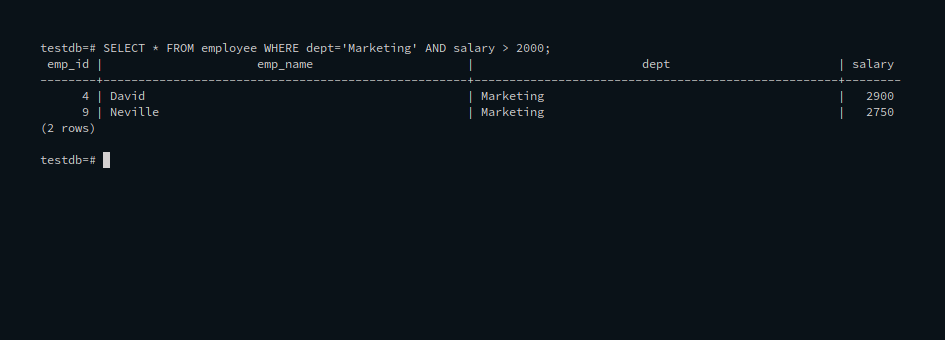
\includegraphics[width=\linewidth]{../Images/Basics/8.png}\newline
\item List the names of all employees working in the sales department and marketing department.\newline
\begin{minted}{sql}

SELECT emp_name FROM employee 
	WHERE dept='Sales' OR dept='Marketing';

\end{minted}
\newline
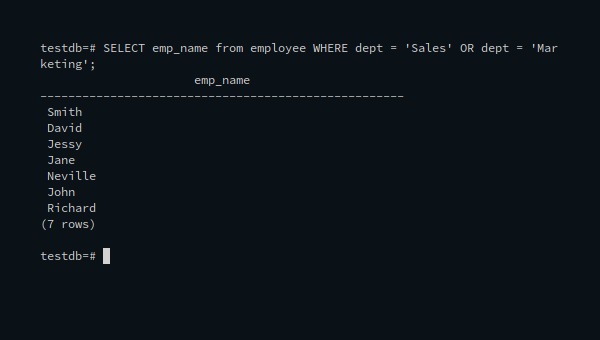
\includegraphics[width=\linewidth]{../Images/Basics/9.png}\newline
\item List the names and department of all employees whose salary is between2300\$ and 3000\$.\newline
\begin{minted}{sql}

SELECT emp_name FROM employee 
	WHERE salary BETWEEN 2300 AND 3000;

\end{minted}
\newline
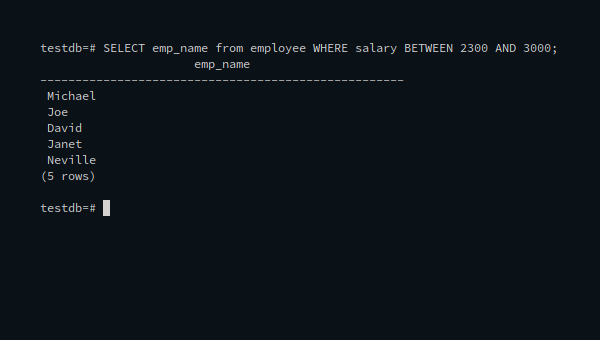
\includegraphics[width=\linewidth]{../Images/Basics/10.png}\newline
\item Update the salary of all employees working in production department 12\%.\newline
\begin{minted}{sql}

UPDATE employee SET salary = salary*1.12 
	WHERE dept='Production';
\end{minted}
\newline
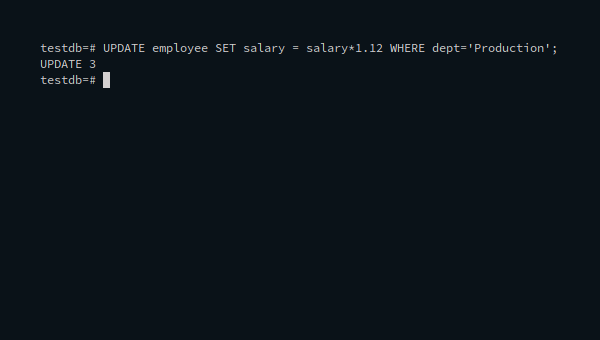
\includegraphics[width=\linewidth]{../Images/Basics/11.png}\newline
\item Display the names of all employees whose salary is less than 2000\$ or working for sales department.\newline
\begin{minted}{sql}

SELECT * FROM employee 
	WHERE salary < 2000 OR dept = 'Sales';

\end{minted}
\newline
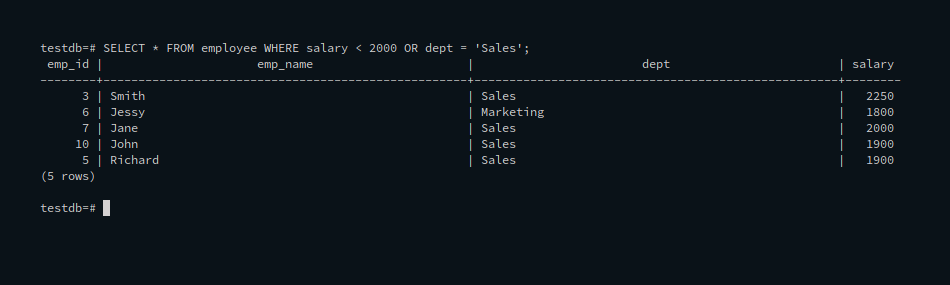
\includegraphics[width=\linewidth]{../Images/Basics/12.png}\newline
\end{enumerate}

\section{Result}
Implemented the program for Basic SQL Queries using Postgresql 11.5 on Manjaro Linux and the output was obtained.